%\chapter{Analysis of Three-dimensional Grain Growth with Surface Tensions}
\chapter{Generation of Two-dimensional statistics from a Three-dimensional Grain Growth Model}
\label{chap:esedoglu}

\lettrine{T}{his} chapter is focused in obtaining two-dimensional statistics from an existing three-dimensional model. 
Esedo\u{g}lu et al.~\cite{Esedoglu2015} presented an algorithm for simulating mean curvature motion of network interfaces in $\mathbb{R}^d$ with arbitrary surface tensions $\sigma$. 
An specific application of this algorithm is precisely grain growth in polycrystalline materials where the interest is focused in $d = 3$ and the two-dimensional statistics that can be generated from slices of the resulting grain structure, as if it were a real bulk of material.

\section{Generation of statistics}
The code that implements the algorithm in~\cite{Esedoglu2015} is available online and implemented in MATLAB at~\cite{esedoglucode}. 
It receives as input a three-dimensional Voronoi tessellation and an array of random orientations, number of iterations, time step size and a grid size. 
The output is the final grain configuration and the related orientations.
% \begin{table}[h]
%     \centering
%     \begin{tabular}{c|c}
%         \hline
%         Parameter & Value\\
%         \hline
%         \hline
%          Number of initial grains &  1000\\
%          Orientations & $\alpha \thicksim \text{Unif}(0,2\pi)$\\
%          Grid dimension & $[0,128]^3$\\
%          \hline
%     \end{tabular}
%     \caption{Parameters used for algorithm presented in \cite{Esedoglu2015}.}
%     \label{table:esedoglu}
% \end{table}

The procedure consists first in perform the numerical simulation and export the resulting grains in \texttt{.mat} format. 
Further post-processing of data is done in Python. The Scipy library allows to import the \texttt{.mat} output and store it as Numpy arrays. 
This output then is interpreted to build the gran surfaces. 
The next step is to generate the slice of the original cube where each grain has to be intersected with a %certain 
plane. 

%Figure \ref{fig:1_cut} shows an initial cut of the grains, a second plane is used to show the cuts in depth.

% \begin{figure}[t]
%     \centering
%     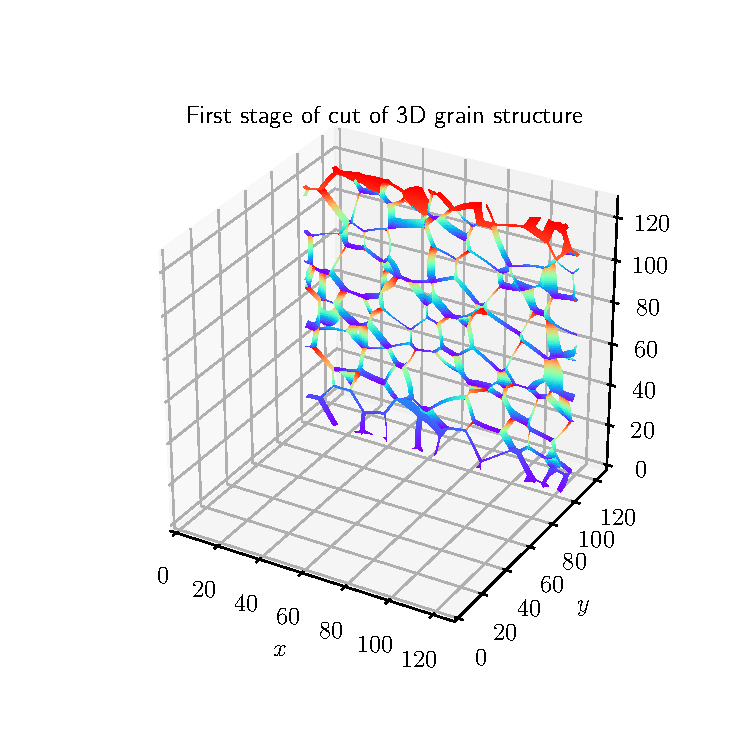
\includegraphics[scale=0.7, trim={0 2em 0 0}]{esedoglu/1_cut.pdf}
%     \caption[Slice of three-dimensional grain cube]{Slice of a cubic grain structure at level $y=100$. An extra plane was added at $y=102$ to clearly show the faces.}
%     \label{fig:1_cut}
% \end{figure}

A larger grid is desirable for simulations, but this requires more memory to store the grain configuration. 
Therefore the initial cut is expanded by some factor to obtain a larger slice. 
Knowing the plane we want to obtain, we recover the discrete data that lies in this plane, obtaining a clean two dimensional description as shown in Figure~\ref{fig:2_discrete}.

\begin{figure}[t]
    \centering
    \subfloat[]{
        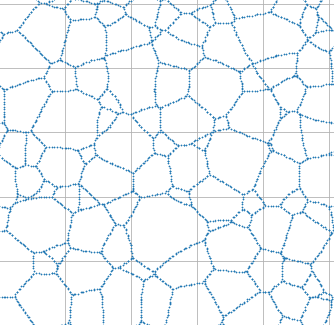
\includegraphics[width=11em]{figures/esedoglu/673_example3.png}
        \label{fig:2_discrete}
    }%
    \subfloat[]{
        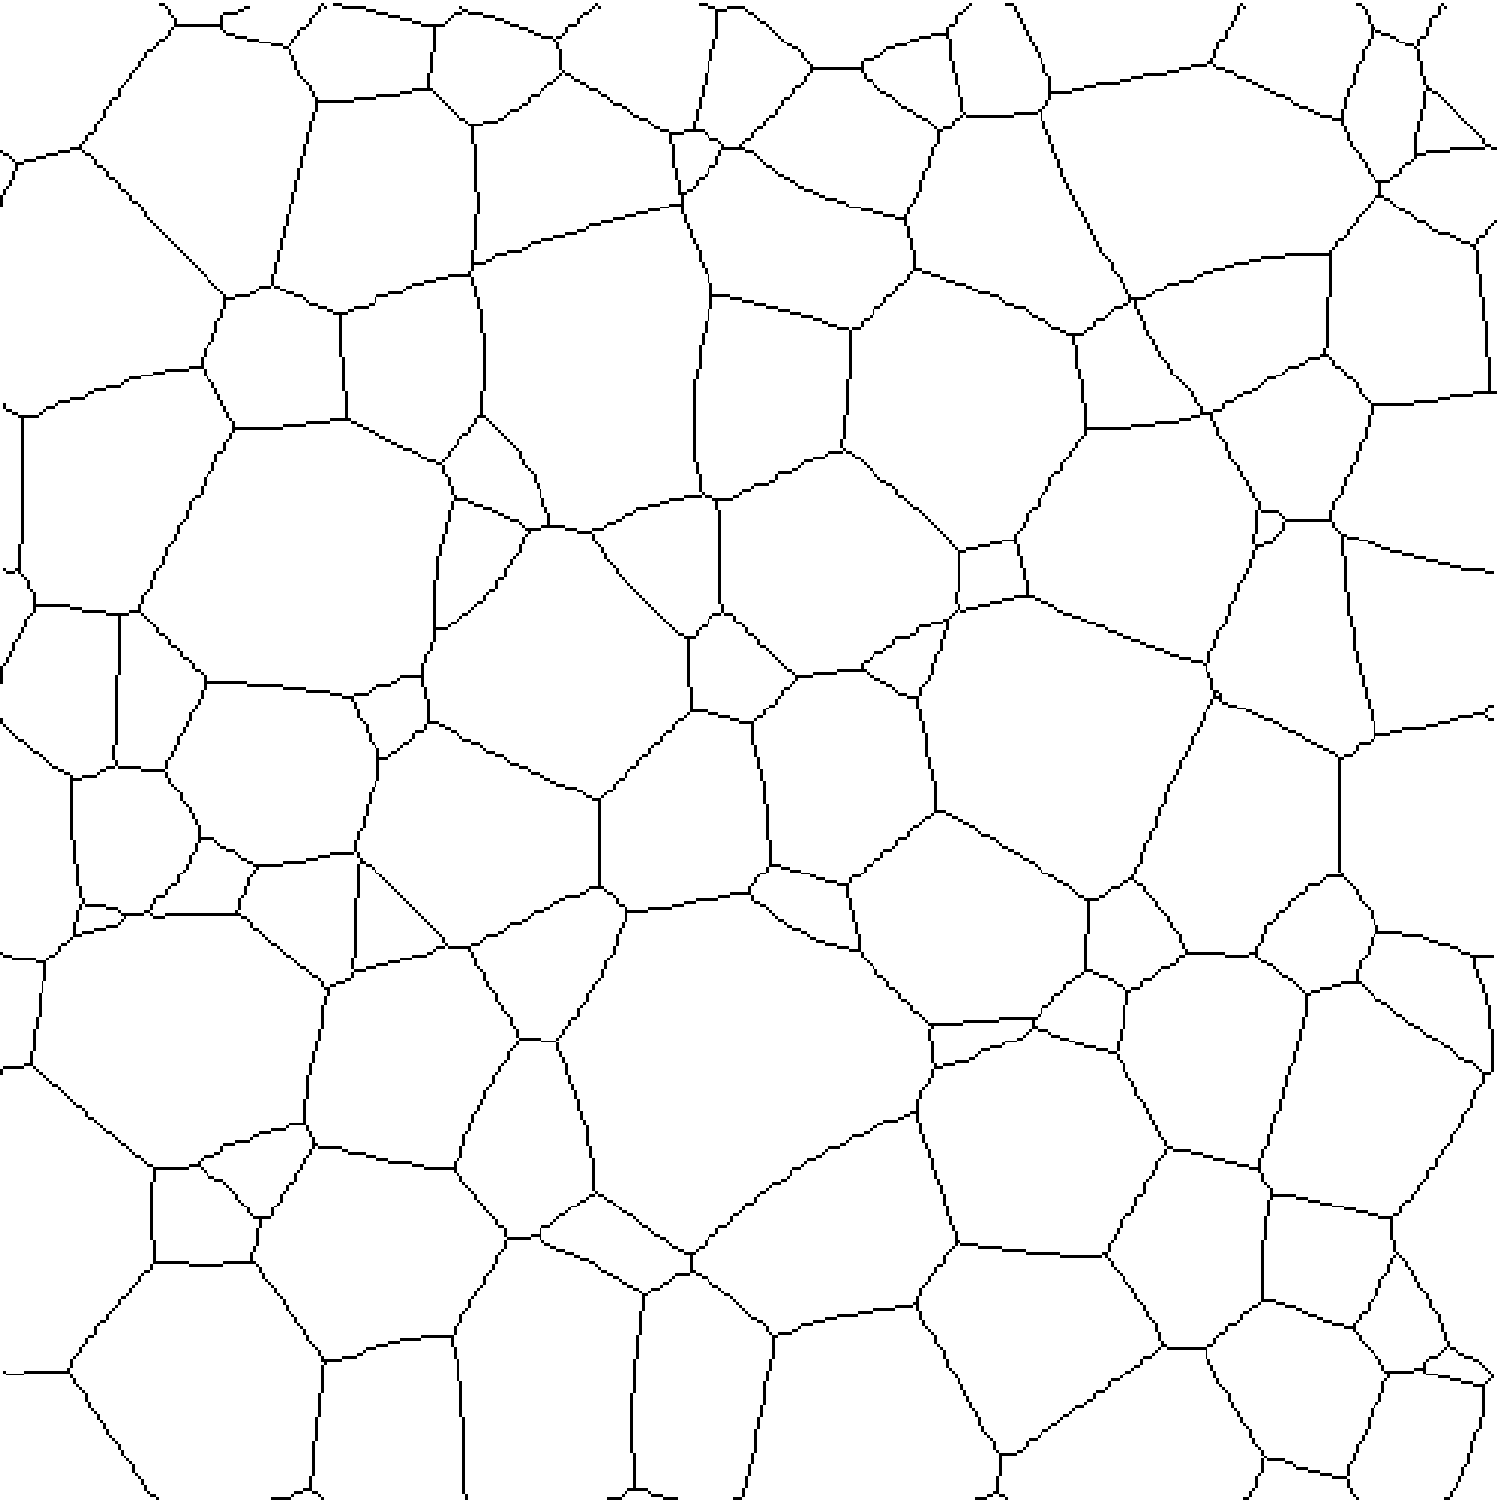
\includegraphics[width=11em, trim={0 0em 0 0em}]{esedoglu/3_full_cut.pdf}
        \label{fig:3_fullcut}
    }%
    \subfloat[]{
        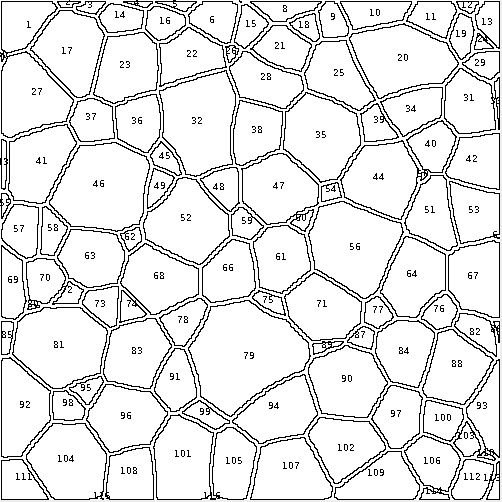
\includegraphics[width=11em, trim={0 0em 0 0}]{esedoglu/4_grains.png}
        \label{fig:4_grains}
    }
    \caption{Discrete and continuous representations of the two-dimensional slide obtained from the three-dimensional simulation.}
\end{figure}

In order to generate a representation with complete boundaries, \ie without discontinuities along boundaries, the obtained data is processed with two image analysis tools: \emph{dilation} and \emph{skeletonize}. 
Dilation operation allows the structure to fulfill the spaces between elements in grain boundaries, but this generates very thick boundaries. Skeletonize operation allows to obtain the skeleton of the dilated image, obtaining a clean picture of grain boundaries as shown in Figure~\ref{fig:3_fullcut}. 
Under the same idea of reduce computation, several cuts of this kind are extracted from the cube over the $x, y$ and $z$-axis.

Using the image analysis software ImageJ~\cite{schneider2012nih} we can obtain statistics of grain structure. 
An internal processing must be done before computing statistics, the image must be converted to 8-bit and binarized to obtain a black-white image easier to analyze. 
ImageJ can detect grains obtain their areas as shown in Figure~\ref{fig:4_grains}. 
Notice that the obtained areas does not consider periodic boundary conditions.

\section{Numerical Experiments}

Experiments were performed with \numprint{1000} initial grains and \numprint{1000} random orientations with distribution $\alpha \thicksim \text{Unif}(0,2\pi)$, running 10 time-steps of size $\Delta t = 5\cdot10^{-4}$ with a computational cubic grid of size $128^3$, which left at the end approximately $500$ grains. 
In order to extract statistics, six runs of the simulation were performed, each time with different initial conditions. 
ImageJ allows to obtain grain areas easily.

Figure~\ref{fig:esedoglu_grains_1} shows the grain relative area distribution after simulation. 
In this simulation the surface tensions -or grain boundary energy- are all equal to 1, which is an isotropic case. 
It is clear that the distribution is not log-normal since accumulates small grains which can be seen at the left of the log scale plot.

Figure~\ref{fig:esedoglu_grains_2} shows the grain relative area distribution after simulation. In this simulation the surface tensions, which are the analogue to the grain boundary energy in two dimensions, are given by the Read-Shockley function:
\begin{equation*}
    \gamma(\theta) = \begin{cases}
       \dfrac{\theta}{\theta_1} \left[1-\log\left(\dfrac{\theta}{\theta_1}\right)\right] & \quad \theta \leq \theta_1\\
        1 & \quad  \theta > \theta_1\\ 
     \end{cases}
\end{equation*}
with $\theta_1 = 15$ is a fixed value and thus only one degree of freedom is used. Again the distribution shows a tail which implies the existence of small grains in the network. We also observe the decrease of grains with relative size close to 1 (bins near 0 in log scale).

The results of the statistics may be affected in part due to image resolution and also by the error introduced by the technique used to obtain the grain area data, which required fine tuning and ignored the periodic boundary condition which may have lead to introduce artificial grain areas.

\begin{figure}[t]
    \centering
    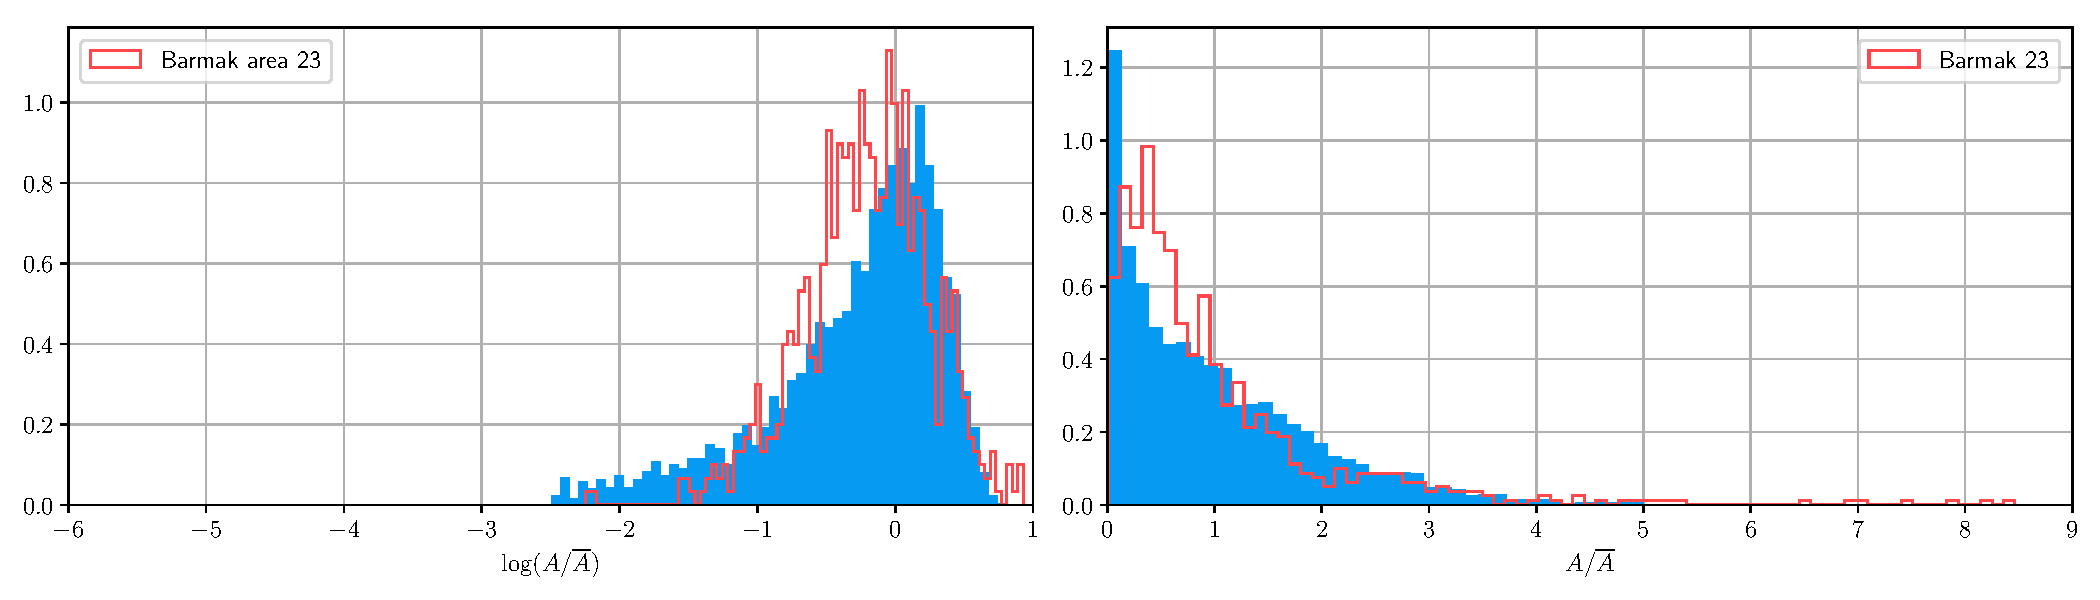
\includegraphics[scale=0.41]{figures/esedoglu/areas_equal.pdf}
    \caption{Distribution of relative areas for two-dimensional cuts with surface tensions equal to 1.}
    \label{fig:esedoglu_grains_1}
\end{figure}

\begin{figure}[t]
    \centering
    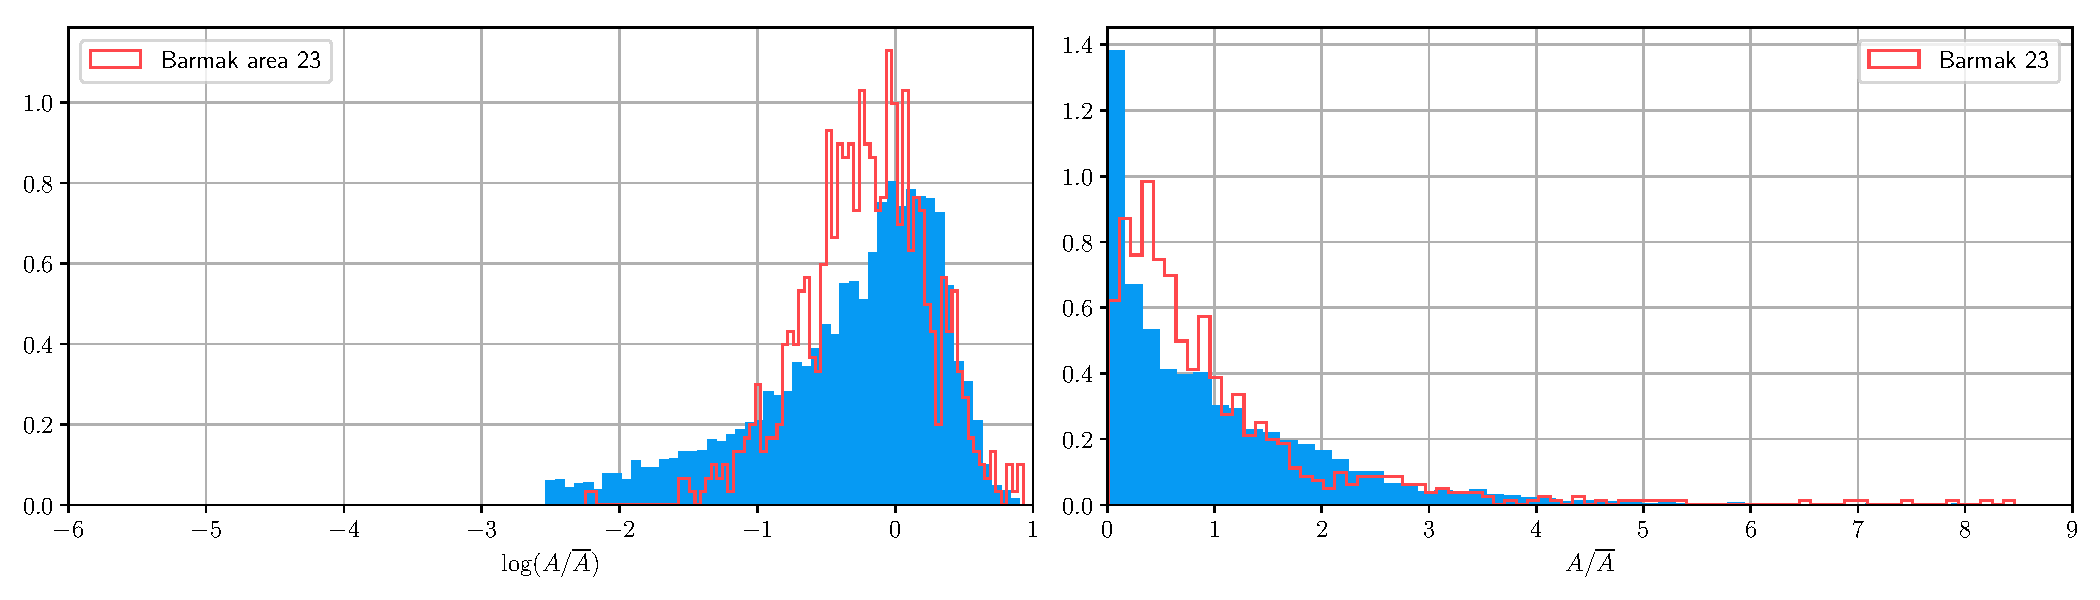
\includegraphics[scale=0.41]{figures/esedoglu/areas_rs.pdf}
    \caption{Distribution of relative areas for two-dimensional cuts with surface tensions obeying Read-Shockley function.}
    \label{fig:esedoglu_grains_2}
\end{figure}
